
\section{Prelude: Fractions}

\begin{minipage}{.55 \textwidth}
Piadina's Restaurant specializes in flatbreads. My favorite is the grilled vegetable flatbread with smoked almond Muhammara (a sauce made from almonds, red bell peppers, red chili peppers, pomegranate molasses, cumin, lemon juice, and olive oil).  Last night I ordered that flatbread and a salad for dinner. They serve each flatbread cut into 5 slices.  
\end{minipage}
\hfill
\begin{minipage}{.4 \textwidth}
\hfill
\scalebox {.45} {\includegraphics [width = 5in] {Flatbread slices.png}}
\vspace{.25in}
\end{minipage}

Turns out the salad was pretty big and so I only ate 3 slides of flatbread.  One way to describe how much of the flatbread I ate is using the fraction $\frac{3}{5}$. 

When I mentioned my dinner to my friend Hayfa she had a strange response:  ``Last time I ate a flatbread at Piadina's I only ate $\frac{2}{3}$ of what you ate.'' I quickly figured it out that since I ate 3 slices and she ate $\frac{2}{3}$ of that, she must have eaten 2 slices, which we can calculate as
$$\frac{2}{3} \times 3 = 2 \div 3 \times 3 = 2$$

I started to obsesses over these fractions. Remember that I ate $\frac{3}{5}$ of the flatbread and Hayfa ate $\frac{2}{3}$ of what I ate.  So she must have eaten $\frac{2}{3}$ of $\frac{3}{5}$, right?  That means
$$ \frac{2}{3} \times \frac{3}{5} = \frac{2}{5}$$
Ah yes!  She ate 2 out of 5 slices, or $\frac{2}{5}$ of the flatbread. That's correct. 

You might remember that we multiply fractions by multiplying the numerator (top) and the denominator (bottom). Let's do that
$$ \frac{2}{3} \times \frac{3}{5} = \frac{2 \times 3}{3 \times 5} = \frac{6}{15}$$
Uh oh.  We got a different answer.

Wait a minute.  Check it out:  
$$ \frac{2}{5} = 2 \div 5 = .4 \text{ \quad and \quad}  \frac{6}{15} = 6 \div 15 = .4$$
Whew!  The fractions $\frac{2}{5} $ and $\frac{6}{15}$ are equal. 

\newpage %%%%%

\noindent
\begin{minipage}{.55 \textwidth}
To see why, consider what happens when I cut the flatbread the other direction twice.  Now the entire flatbread has 15 squares.  Hayfa ate 2 slices out of the original 5 slices total.  Or, equivalently, she at 6 squares out of 15 original squares. You may have heard of reducing or cancelling fractions, which is a way to remember what's happening here:
\end{minipage}
\hfill
\begin{minipage}{.4 \textwidth}
\hfill
\scalebox {.45} {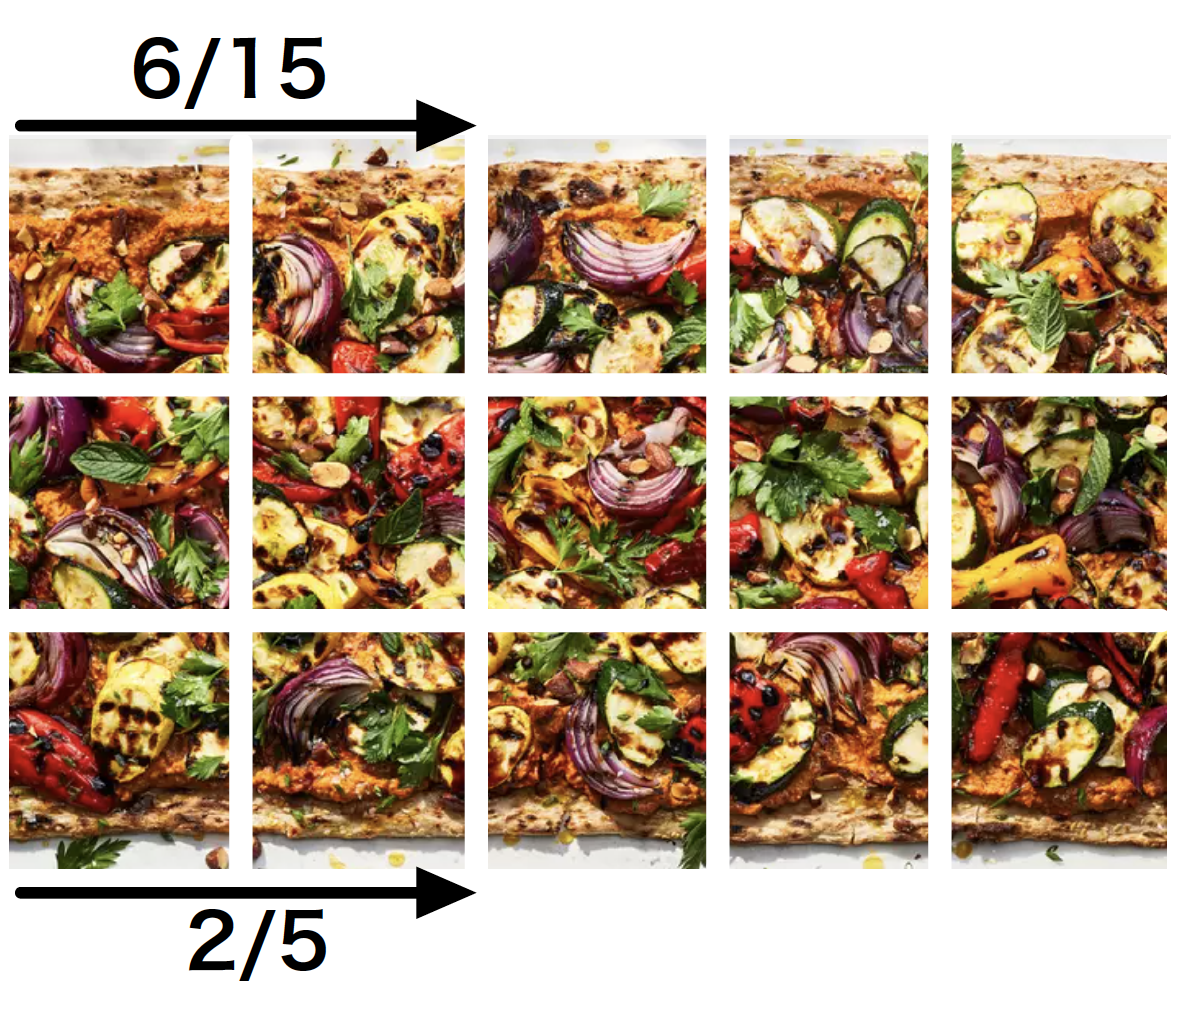
\includegraphics [width = 5in] {Flatbread squares.png}}
\vspace{.25in}
\end{minipage}
\vspace{-.3in}

$$\frac{2 \times 3}{3 \times 5} = \frac{2 \times \cancel{~3~}}{ \cancel{~3~} \times 5} = \frac{2}{5}$$

In practice when we have to evaluate a product of fractions we can do it a couple of ways.  One way is to deal with each fraction separately:

$$\frac{2}{3} \times \frac{3}{5} = 2 \div 3 \times 3 \div 5 = .4$$

Another way is to calculate the top and bottom of the fraction and divide.  Notice how we need to use parentheses around the top and bottom of the fraction.

$$ \frac{2}{3} \times \frac{3}{5} = \frac{2 \times 3}{3 \times 5} = (2 \times 3)\div (3 \times 5) = .4$$

By the way, flatbreads at Piadina's are pricey:  \$17.49 each.  At that rate, what does each slice cost?  We can use a fraction
$$\frac{\$17.49}{5 \text{ slices}} = \$17.49 \div 5 = 3.498 \approx \$3.50 \text{ per slice}$$
Notice that the units on my answer are dollars per slice:  the units of the numerator (top) per the units of the denominator (bottom).  We sometimes even write the units themselves as a fraction: $\frac{\$}{\text{slice}}$

There will be a few times during this course where you encounter fractions.  Mostly we'll switch to decimal approximations right away.  

 \begin{center}
\line(1,0){300} %\line(1,0){250}
\end{center}

\section*{Homework}

\noindent \textbf{Start by doing Practice exercises \#1-4 in the workbook.}

\bigskip

\noindent \textbf{Do you know \ldots}

\begin{itemize} 
\item How we represent a part of a whole as a fraction? %\vfill
\item How to multiply fractions?  %\vfill
\item What``canceling'' a factor means? %\vfill
\item How fractions are related to division? %\vfill
\item How to calculate the decimal approximation of a fraction? %\vfill
\item How to compare two fractions using their decimal approximations? %\vfill
\item How the units of a fraction are determined?  %\vfill
\item When we need to use parentheses around the top (numerator) and bottom (denominator) to evaluate a fraction? %\vfill
 \item[~] \textbf{If you're not sure, work the rest of exercises and then return to these questions.  Or, ask your instructor or a classmate for help.} 
\end{itemize}

\subsection*{Exercises}

On each problem, write down what you enter into your calculator and don't forget to write the units on your final answer.  Challenge yourself to use one-line calculations. You are welcome to calculate the answer step-by-step to check.

\begin{enumerate} 
\setcounter{enumi}{4}

\item In our flatbread example, the flatbread was served cut into 5 slices and we cut it lengthwise into 15 squares. 
\begin{enumerate}
\item Use our flatbread example to explain why $\frac{12}{15} = \frac{4}{5}$ and confirm by calculating the decimals. 
\item Use our flatbread example to explain why $\frac{10}{15} = \frac{2}{3}$ (hint:  think of very long strips!) and confirm by calculating the decimals.
\end{enumerate}

\item Auriel is making porridge but doesn't want too much.  Last time she cut the recipe in half, but that was too little. Auriel has decided that making $\frac{3}{4}$ of the recipe will be just right.  Figure out how much of each ingredient Auriel needs.  Report each answer as both a fraction and a decimal.

\begin{enumerate}
\item The original recipe calls for 5 ounces of skim milk.
\item The original recipe calls for $\frac{1}{2}$ cup oats.
\item The original recipe calls for $\frac{2}{3}$ cup of water.
\item The original recipe calls for $\frac{1}{3}$ cup of raisins.  
\end{enumerate}

\item A diver bounces on a 3-meter springboard.  Up she goes.  A somersault, a twist, and then whoosh, into the water.  \hfill \emph{Story also appears in 1.3.}
\begin{enumerate}
\item At .2 seconds after take-off she was 3.88 meters above the water.  Her initial speed can be calculated as 
$$\frac{3.88-3}{.2}$$
Find the diver's speed and don't forget the units.
\item At .4 seconds after take-off she was 4.38 meters above the water.  Her speed then can be calculated as 
$$\frac{4.38-3.88}{.4-.2 }$$
Find the diver's speed and don't forget the units.
\item Which speed is larger? Explain why that might make sense in the story.
\end{enumerate}

\item The football coach wants everyone to sprint three-quarters of a mile, up and back on the field which is labeled in years.  \hfill \emph{Story appears in 1.4 \#7.}
\begin{enumerate}
\item Find the number of yards by calculating
$$\frac{3}{4} \text{ miles}
\star
  \frac{\text{5,280} \text{ feet}}{1 \text{ mile}}
\star
  \frac{\text{1} \text{ yard}}{3 \text{ feet}} = \frac{3 \times 5280}{4 \times 3}$$
  \item Approximately how many times will the players need to run up and back on the field.  The field is 100 yards long so ``up and back'' is 200 yards.  
  \end{enumerate}



  


\end{enumerate}

\bigskip

\noindent \textbf{When you're done \ldots}

\begin{itemize}
\item Don't forget to check your answers with those in the back of the textbook. 
\item Not sure if your answers are close enough? Compare with a classmate or ask the instructor.  
\item Getting the wrong answers or stuck on a problem?  Re-read the section and try the problem again.   If you're still stuck, work with a classmate or go to your instructor's office hours.
\item It's normal to find some parts of some problems difficult, but if all the problems are giving you grief, be sure to talk with your instructor or advisor about it.  They might be able to suggest strategies or support services that can help you succeed.
\item Make a list of key ideas or processes to remember from the section.  The ``Do you know?'' questions can be a good starting point.
\end{itemize}

